\documentclass{article}

% if you need to pass options to natbib, use, e.g.:
%     \PassOptionsToPackage{numbers, compress}{natbib}
% before loading neurips_2020

% ready for submission
% \usepackage{neurips_2020}

% to compile a preprint version, e.g., for submission to arXiv, add add the
% [preprint] option:
%     \usepackage[preprint]{neurips_2020}

% to compile a camera-ready version, add the [final] option, e.g.:
    \usepackage[final]{neurips_2020}

% to avoid loading the natbib package, add option nonatbib:
     % \usepackage[nonatbib]{neurips_2020}

\usepackage[utf8]{inputenc} % allow utf-8 input
\usepackage[T1]{fontenc}    % use 8-bit T1 fonts
\usepackage{hyperref}       % hyperlinks
\usepackage{url}            % simple URL typesetting
\usepackage{booktabs}       % professional-quality tables
\usepackage{amsfonts}       % blackboard math symbols
\usepackage{nicefrac}       % compact symbols for 1/2, etc.
\usepackage{microtype}      % microtypography

%% Customized package by Mao Song
\usepackage{listings}
\usepackage{graphicx}
\usepackage{amsthm}
\usepackage{amsmath}
\newcommand*\diff{\mathop{}\!\mathrm{d}}
\theoremstyle{definition}
\newtheorem{solution}{Solution}

\usepackage{xcolor}

\definecolor{codegreen}{rgb}{0,0.6,0}
\definecolor{codegray}{rgb}{0.5,0.5,0.5}
\definecolor{codepurple}{rgb}{0.58,0,0.82}
\definecolor{backcolour}{rgb}{0.95,0.95,0.92}

\lstdefinestyle{mystyle}{
    backgroundcolor=\color{backcolour},   
    commentstyle=\color{codegreen},
    keywordstyle=\color{magenta},
    numberstyle=\tiny\color{codegray},
    stringstyle=\color{codepurple},
    basicstyle=\ttfamily\footnotesize,
    breakatwhitespace=false,         
    breaklines=true,                 
    captionpos=b,                    
    keepspaces=true,                 
    numbers=left,                    
    numbersep=5pt,                  
    showspaces=false,                
    showstringspaces=false,
    showtabs=false,                  
    tabsize=2
}

\lstset{style=mystyle}


\title{Homework 5 for SI211: Numerical Analysis}

% The \author macro works with any number of authors. There are two commands
% used to separate the names and addresses of multiple authors: \And and \AND.
%
% Using \And between authors leaves it to LaTeX to determine where to break the
% lines. Using \AND forces a line break at that point. So, if LaTeX puts 3 of 4
% authors names on the first line, and the last on the second line, try using
% \AND instead of \And before the third author name.

\author{%
  {Mao Song} \\
  SIST\\
  ShanghaiTech University\\
  Student ID: 2019233134 \\
  \texttt{maosong@shanghaitech.edu.cn} \\
}

\begin{document}

\maketitle

\begin{abstract}
  This is the solution for Homework 5 of SI211: Numerical Analysis, which is taught by Boris Houska.

\end{abstract}

\section{Probelm 1}
The goal of this exercise is to compare different methods for approxi-
mating the integral
\begin{equation}
	\int_{0}^{4}e^x\diff x
\end{equation}
For this aim, we first write the integral in the form
\begin{equation}
	\int_{0}^{4}e^x\diff x=\sum_{i=0}^{N-1}\left\{\int_{4i/N}^{4(i+1)/N}e^x\diff x\right\}
\end{equation}
then apply Simpson’s rule on each of the integrals separately, and sum
up the result.
\begin{enumerate}
	\item Plot the actual error of the integral approximation versus $N$ for $N \in \{0, 1, 2, \dots, 100\}$.
	\item Derive a theoretical bound on the integral approximation in dependence on N and plot this upper bound, too.
\end{enumerate}


\begin{solution}
	\begin{enumerate}
		\item The solution is shown as Fig \ref{Fig:solution_to_problem1}.
		\item By Simpson Rule:
		\begin{align*}
		\int_{a}^{b}f(x)\diff x&=\frac{b-a}{6}\left[f(a)+4f\left(\frac{a+b}{2}\right)+f(b)\right]-\frac{(b-a)^5}{2880}f^{(4)}(\xi),\xi\in(a,b)\\
		&:=I_{[a,b]}-\frac{(b-a)^5}{2880}f^{(4)}(\xi),\xi\in(a,b)
		\end{align*}
		
		Denote $x_i=4i/N$ and $x_{i+1}=4(i+1)/N$,  we have
		\begin{align*}
		\int_{0}^{4}e^x\diff x&=\sum_{i=0}^{N-1}\left\{\int_{x_i}^{x_{i+1}}e^x\diff x\right\}\\
		&=\sum_{i=0}^{N-1}\left\{I_{[x_i,x_{i+1}]}-\frac{16}{45N^5}\exp(\xi_i)\right\}. \xi_i\in\left(x_i,x_{i+1}\right)\\
		&=\sum_{i=0}^{N-1}I_{[x_i,x_{i+1}]}-\frac{16}{45N^5}\sum_{i=0}^{N-1}\exp(\xi_i)
		\end{align*}
		which implies
		\begin{align*}
		\Big|\int_{0}^{4}e^x\diff x-\sum_{i=0}^{N-1}I_{[x_i,x_{i+1}]}\Big|&=\frac{16}{45N^5}\sum_{i=0}^{N-1}\exp(\xi_i)\\
		&\leq \frac{16}{45N^5}\sum_{i=0}^{N-1}\exp(x_{i+1})\\
		&=\frac{16p(1-p^N)}{45N^4(1-p)}
		\end{align*}
		where $p=\exp(\frac{4}{N})$. The plot with the bound are shown in Fig \ref{Fig:bounds}. 

	\end{enumerate}
	\begin{figure}[ht]
      \label{Fig:solution_to_problem1}
      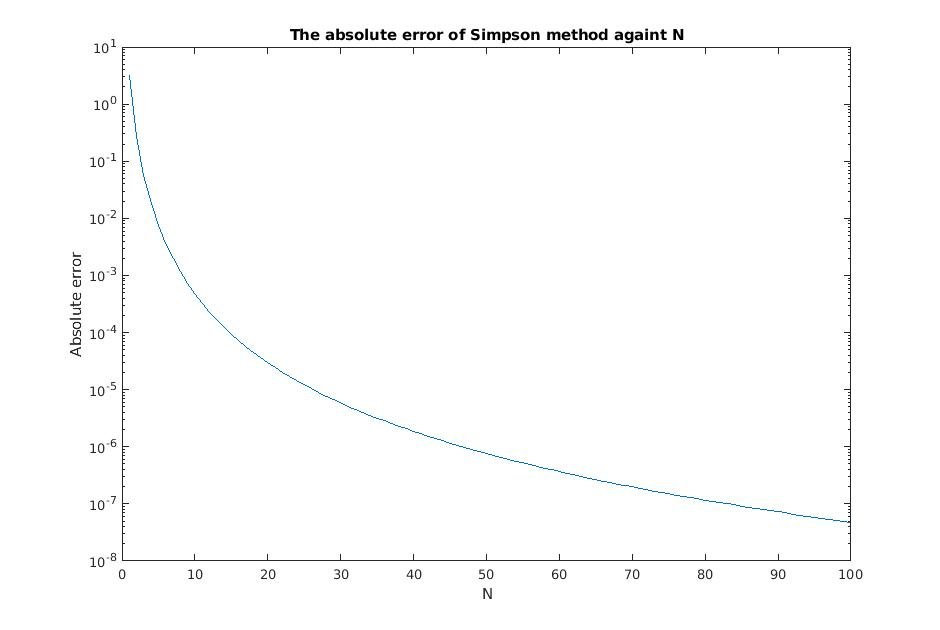
\includegraphics[width=0.8\textwidth]{solution_to_problem1.jpg}
      \centering
      \caption{The absolute error of Simpson method against $N$}
    \end{figure}
    \begin{figure}[ht]
      \label{Fig:bounds}
      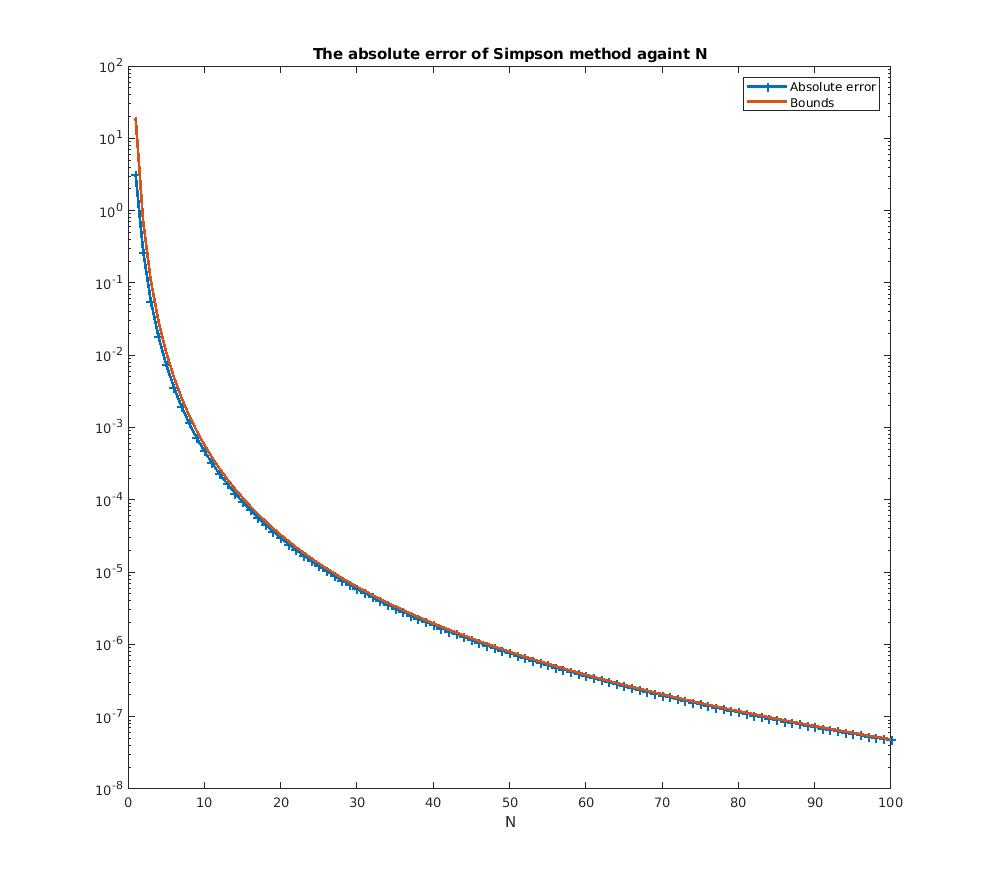
\includegraphics[width=0.8\textwidth]{bounds.jpg}
      \centering
      \caption{The absolute error of Simpson method against $N$}
    \end{figure}
\end{solution}

\section{Probelm 2}
Implement and compare the results of the closed Newton-Cotes formulas for $n = 3$ and $n = 5$ when approximating the integral
\begin{equation}
	\int_{0}^{\pi/4}\sin(x)\diff x=1-\frac{\sqrt{2}}{2}
\end{equation}

\begin{solution}
	Let $f(x)=\sin(x)$.
	For $n=3$, we have $h=(\frac{\pi}{4}-0)/3=\frac{\pi}{12}$, $x_0=0$, $x_1=\frac{\pi}{12}$, $x_2=\frac{\pi}{6}$, $x_3=\frac{\pi}{4}$. then
	\begin{align*}
	\int_{0}^{\frac{\pi}{4}}\sin(x)\diff x&\approx \frac{3h}{8}\left[f(x_0)+3f(x_1)+3f(x_2)+f(x_3)\right]\\
	&=0.29291070
	\end{align*}
	The error is bounded by 
	\begin{equation}
		\varepsilon_{n=3}\leq \Big|\frac{3h^5}{80}f^{(4)}(\xi)\Big|=\Big|\frac{3h^5\pi^5}{80*12^5}\cos(\xi)\Big|\leq \Big|\frac{3\pi^5}{80*12^5}\Big|\approx 0.00004611
	\end{equation}
	For $n=5$, we have $h=(\frac{\pi}{4}-0)/5=\frac{\pi}{20}$, $x_0=0$, $x_1=\frac{\pi}{20}$, $x_2=\frac{\pi}{10}$, $x_3=\frac{3\pi}{20}$, $x_4=\frac{\pi}{5}$, $x_5=\frac{\pi}{4}$. then
	\begin{align*}
	\int_{0}^{\frac{\pi}{4}}\sin(x)\diff x&\approx \frac{5h}{288}\left[19f(x_0)+75f(x_1)+50f(x_2)+50f(x_3)+75f(x_4)+19f(x_5)\right]\\
	&=0.29289320
	\end{align*}
	The error is bounded by
	\begin{equation}
		\varepsilon_{n=5}\leq \Big|\frac{275h^7}{12096}f^{(6)}(\xi)\Big|=\Big|\frac{275\pi^7}{12096*12^7}\cos(\xi)\Big|\leq \Big|\frac{275\pi^7}{12096*20^7}\Big|\approx 0.00000005
	\end{equation}
	The absolute error are
	\begin{align*}
		\varepsilon_{n=3}&=|1-\frac{\sqrt{2}}{2}-0.29291070|=0.00001748\\
		\varepsilon_{n=5}&=|1-\frac{\sqrt{2}}{2}-0.29289320|=0.00000002
	\end{align*}
	We can see that as $n$ becomes large, the error and the error bound become smaller and smaller.
\end{solution}

\section{Probelm 3}
The exact value of the integral
\begin{equation}
	I(\omega)=\int_{0}^{\pi/4}\cos(\omega x)\diff x
\end{equation}
is given by $I(w)=\frac{1}{w}\sin(wx)$ for any $w>0$. In the following, we test
how accurate a Gauss-Quadrature of the form
\begin{equation}
	\label{eq:Gauss-Quadrature}
	I_1(\omega)=\sum_{i=0}^{1}\alpha_i\cos(\omega x_i)
\end{equation}
can approximate this integral. Explain how to compute the approximation $I_1(\omega) \approx I(\omega)$. You may use that the second order $q$ Legendre
polynomial of order $2$ on the interval $[-1,1]$ has root s at $\pm\sqrt{\frac{1}{3}}$. How
large is the approximation error $|I(1)-I_1(1)|$? What happens for large $\omega$? Plot your result.

\begin{solution}
	The first Gauss quadrature formula is given by
	\begin{equation}
		\int_{-1}^{1}f(x)\diff x\approx f\left(-\sqrt{\frac{1}{3}}\right)+f\left(\sqrt{\frac{1}{3}}\right)
	\end{equation}
	which is exact for polynomials of order less or equal than $3$.
	By using the changing of variables:
	\begin{equation}
		t=\frac{8x-\pi}{\pi}\Leftrightarrow x=\frac{1}{2}\left[\frac{\pi}{4}t+\frac{\pi}{4}\right]
	\end{equation}
	we have
	\begin{align*}
	\int_{0}^{\pi/4}\cos(\omega x)\diff x&=\int_{0}^{\pi/4}f(x)\diff x\\
	&=\int_{-1}^{1}f\left(\frac{\pi(t+1)}{8}\right)\frac{\pi}{8}\diff t\\
	&=\frac{\pi}{8}\int_{-1}^{1}g(t)\diff t\\
	&=\frac{\pi}{8}\left[g\left(-\sqrt{\frac{1}{3}}\right)+g\left(\sqrt{\frac{1}{3}}\right)\right]\\
	&=\frac{\pi}{8}\left[f\left(\frac{\pi(\sqrt{3}-1)}{8\sqrt{3}}\right)+f\left(\frac{\pi(\sqrt{3}+1)}{8\sqrt{3}}\right)\right]\\
	&=\frac{\pi}{8}\left[\cos\left(\omega\frac{\pi(\sqrt{3}-1)}{8\sqrt{3}}\right)+\cos\left(\omega\frac{\pi(\sqrt{3}+1)}{8\sqrt{3}}\right)\right]
	\end{align*}
	where $f(x)=\cos(\omega x)$, $g(t)=f\left(\frac{\pi(t+1)}{8}\right)$. Compare with Eq \ref{eq:Gauss-Quadrature}, we have
	\begin{equation}
		\alpha_0=\alpha_1=\frac{\pi}{8}, x_0=\frac{\pi(\sqrt{3}-1)}{8\sqrt{3}}, x_1=\frac{\pi(\sqrt{3}+1)}{8\sqrt{3}}
	\end{equation}
	The approximation error is then given by (notice that $n=1$)
	\begin{equation}
		|I(1)-I_1(1)|\leq \left(\frac{\pi}{4}\right)^4\approx 0.3805
	\end{equation}
	\begin{figure}[ht]
      \label{Fig:error_of_approximation}
      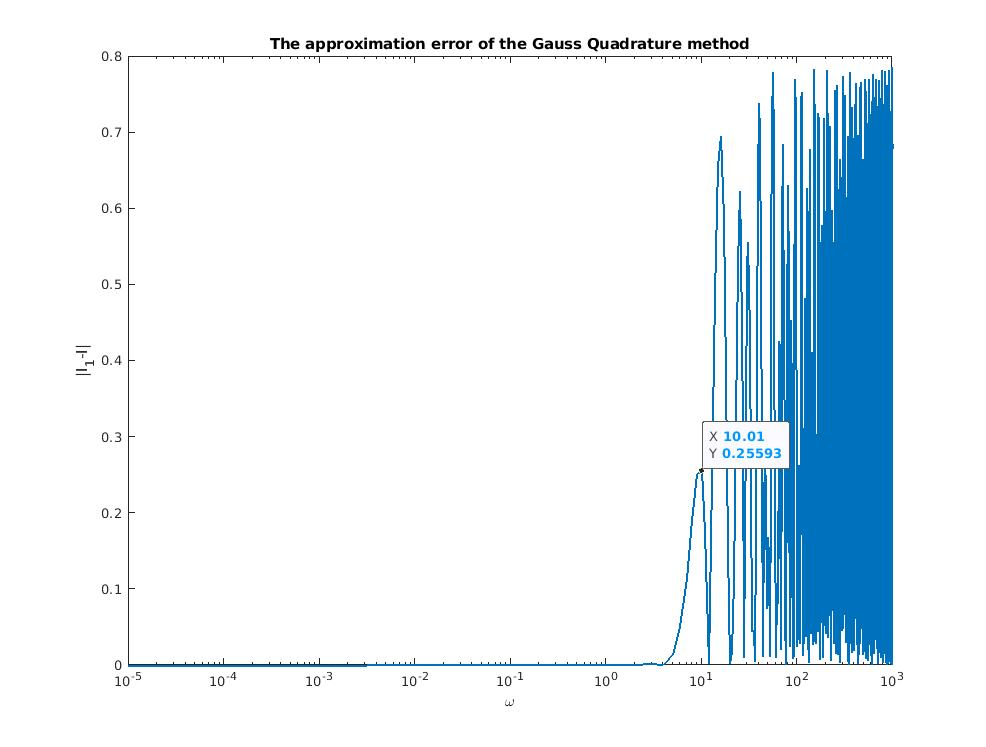
\includegraphics[width=0.8\textwidth]{problem3_error_figure.jpg}
      \centering
      \caption{The error of approximation against $\omega$}
    \end{figure}
    As Fig \ref{Fig:error_of_approximation} shows, the error becomes large when $\omega$ becomes large, when $\omega>10$, the error bound is meaningless, let's see the figure of exact solution and the approximate solution:
    \begin{figure}[ht]
      \label{Fig:solution_of_approximation}
      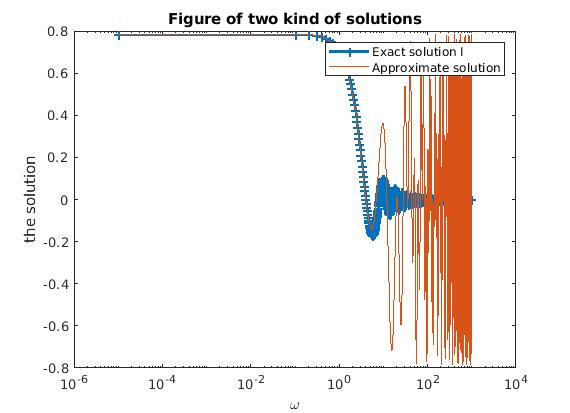
\includegraphics[width=0.8\textwidth]{problem3_solution_figure.jpg}
      \centering
      \caption{The figure of two kinds of solution against $\omega$}
    \end{figure}
    As is can be seen from Fig \ref{Fig:solution_of_approximation}, the exact solution is approximating the function $h(\omega)=\frac{1}{\omega}$, but the approximate solution changes as $\omega$ changes since it's a $\cos$ function of $\omega$. In a word, when $\omega$ is relative small ($\omega<10$), the approximation is accurate (the bound is meaningful). When $\omega$ is large, the approximation will fail.
\end{solution}

\section{Probelm 4}
We would like to develop a new numerical integration formula by passing through the following steps:
\begin{enumerate}
	\item compute the coefficients $c_1,\dots,c_2,c_3$ such that
	\begin{equation}
		\forall i\in\{1,2,3\}, \quad f(x_i)=c_1+c_2\sin(x_i)+c_3\cos(x_i)
	\end{equation}
	for $x_1=a, x_2=\frac{a+b}{2}$, and $x_3=b$. You may assume that $b>a$ as well as $b-a<\frac{\pi}{2}$.
	\item Derive an integral approximation of the form
	\begin{equation}
		\int_{a}^{b}f(x)\diff x\approx \int_{a}^{b}\left[c_1+c_2\sin(x)+c_3\cos(x)\right]\diff x
	\end{equation}
	by working out an explicit expression for the integral on the right side.
	\item Combine the above two results to show that the final numerical integration formula can be written in the form
	\begin{equation}
		\int_{a}^{b}f(x)\diff x\approx \alpha_1f(a)+\alpha_2f\left(\frac{a+b}{2}\right)+\alpha_3f(b)
	\end{equation}
	What are the coefficients $\alpha_1,\alpha_2,\alpha_3$?
\end{enumerate}
Compare the above integration formula with Simpson’s formula for the
integrals
\begin{equation}
	\int_{0}^{0.5}\sin\left(\frac{9}{10}x\right)\diff x, \int_{0}^{1}x^3\diff x\text{ and }\int_{0}^{1}\cos(x)\diff x 
\end{equation}
Which integration formula is better? Discuss advantages and disadvantages.



\begin{solution}
	From step 1, $c_1,c_2,c_3$ are given by
	\begin{equation}
		\begin{bmatrix}
			1& \sin(a)& \cos(a)\\
			1& \sin(\frac{a+b}{2})& \cos(\frac{a+b}{2})\\
			1& \sin(b)& \cos(b)
		\end{bmatrix}\begin{bmatrix}
			c_1\\
			c_2\\
			c_3
		\end{bmatrix}=\begin{bmatrix}
			f(a)\\
			f(\frac{a+b}{2})\\
			f(b)
		\end{bmatrix}
	\end{equation}

	By the integral approximation form, we have
	\begin{equation}
		\int_{a}^{b}f(x)\diff x\approx c_1(b-a)+c_2(\cos(a)-\cos(b))+c_3(\sin(b)-\sin(a))
	\end{equation}
	By step 3, we have
	\begin{align}
	\int_{a}^{b}f(x)\diff x&\approx\alpha_1 f(a)+\alpha_3f(\frac{a+b}{2})+\alpha_3f(b)\\
	&=\alpha_1\left[c_1+c_2\sin(a)+c_3\cos(a)\right]+\alpha_2\left[c_1+c_2\sin(\frac{a+b}{2})c_3\cos(\frac{a+b}{2})\right]\\
	&\quad +\alpha_3\left[c_1+c_2\sin(b)+c_3\cos(b)\right]\\
	&=c_1(b-a)+c_2(\cos(a)-\cos(b))+c_3(\sin(b)-\sin(a))
	\end{align}
	By collecting terms according to $f(a)$, $f\left(\frac{a+b}{2}\right)$, $f(b)$ in equation (19-21), we can obtain $\alpha_1,\alpha_2,\alpha_3$.

	\begin{align*}
		\alpha_1=&\frac{\cos(x_1 - x_2) - \cos(x_1 - x_3) - \cos(x_2 - x_3) - x_1\sin(x_2 - x_3) + x_3\sin(x_2 - x_3) + 1}{\sin(x_1 - x_2) - \sin(x_1 - x_3) + \sin(x_2 - x_3)}\\
		\alpha_2=&\frac{2\cos(x_1 - x_3) + x_1\sin(x_1 - x_3) - x_3\sin(x_1 - x_3) - 2}{\sin(x_1 - x_2) - \sin(x_1 - x_3) + \sin(x_2 - x_3)}\\
		\alpha_3=&-\frac{\cos(x_1 - x_2) + \cos(x_1 - x_3) - \cos(x_2 - x_3) + x_1\sin(x_1 - x_2) - x_3\sin(x_1 - x_2) - 1}{\sin(x_1 - x_2) - \sin(x_1 - x_3) + \sin(x_2 - x_3)}
	\end{align*}
	After substituting $x_1=a$, $x_2=(a+b)/2$, $x_3=b$, we have
	\begin{align*}
	\alpha_1 &= -\frac{\cos(a - b) + a\sin(a/2 - b/2) - b\sin(a/2 - b/2) - 1}{2\sin(a/2 - b/2) - \sin(a - b)}\\
	\alpha_2 &= \frac{2\cos(a - b) + a\sin(a - b) - b\sin(a - b) - 2}{2\sin(a/2 - b/2) - \sin(a - b)}\\
	\alpha_3 &= -\frac{\cos(a - b) + a\sin(a/2 - b/2) - b\sin(a/2 - b/2) - 1}{2\sin(a/2 - b/2) - \sin(a - b)}
	\end{align*}
	
	Denote $I_1$ as the above approximation integration, $I_2$ the Simpson's method, $I$ the exact value of integration. For $f(x)=\sin(\frac{9x}{10})$, we have
	\begin{equation}
		I=0.11061433,\quad I_1=0.11061396,\quad I_2=0.11061592
	\end{equation}
	The error is given by
	\begin{equation}
		\varepsilon_1 = |I_1-I|=3.7*10^{-7}, \quad \varepsilon_2 = |I_2-I|=1.59*10^{-6}
	\end{equation}
	For $g(x)=x^3$, we have
	\begin{equation}
		I=0.25000000,\quad I_1=0.25105105,\quad I_2=0.25000000
	\end{equation}
	The error is given by
	\begin{equation}
		\varepsilon_1 = |I_1-I|=1*10^{-3}, \quad \varepsilon_2 = |I_2-I|=0
	\end{equation}
	For $h(x)=\cos(x)$, we have
	\begin{equation}
		I=0.84147098, \quad I_1=0.84147098, \quad I_2=0.84177209
	\end{equation}
	The error is given by
	\begin{equation}
		\varepsilon_1 = |I_1-I|=0, \quad \varepsilon_2 = |I_2-I|=3*10^{-4}
	\end{equation}
	From the above results, we can see that when the function is trigonometric function ($\sin(x),\cos(x)$), the proposed approximation formula performs better than the Simposon method; when the function is a polynomial function, the Simpson method performs better than the proposed approximation formula. The reason is that we use $1,\cos(x),\sin(x)$ to form a basis while the Simposon method use the $1,x,x^2,\dots$ to form a basis, when the function lies in different space, the corresponding method will be well-behaviored.
\end{solution}



\end{document}
